\documentclass[10pt,twocolumn,letterpaper]{article}
\usepackage{comment}

\usepackage[utf8]{inputenc}
\usepackage{caption}
\usepackage{tabularx}
\captionsetup[table]{skip=20pt}
\captionsetup{hypcap=false}
\usepackage{cvpr}
\usepackage{epsfig}
\usepackage{graphicx}
\usepackage{graphicx}
\usepackage{amsmath}
\usepackage{siunitx}
\usepackage{physics}
\usepackage{amssymb}
\usepackage{tikz}
\usepackage{pgfplots}
\usepackage{subcaption}
\usepackage{bm,color}
\usetikzlibrary{arrows.meta, shadings, shadows, shapes, arrows}
\usepackage{graphics}
\usepackage{pifont}
\pgfplotsset{compat=newest}
\usepackage{comment}

\usepackage[pagebackref=true,breaklinks=true,colorlinks,bookmarks=false]{hyperref}

\newcommand{\cmark}{\ding{51}}
\newcommand{\xmark}{\ding{55}}

% Input TU-Darmstadt colors
\definecolor{tud0d}{cmyk/RGB/HTML}{0,0,0,.8/83,83,83/535353}
\definecolor{tud0c}{cmyk/RGB/HTML}{0,0,0,.6/137,137,137/898989}
\definecolor{tud0b}{cmyk/RGB/HTML}{0,0,0,.4/181,181,181/B5B5B5}
\definecolor{tud0a}{cmyk/RGB/HTML}{0,0,0,.2/220,220,220/DCDCDC}
\definecolor{tud1a}{cmyk/RGB/HTML}{.7,.4,0,0/93,133,195/5D85C3}
\definecolor{tud2a}{cmyk/RGB/HTML}{0.8,.2,0,0/0,156,218/009CDA}
\definecolor{tud3a}{cmyk/RGB/HTML}{0.7,0,.5,0/80,182,149/50B695}
\definecolor{tud4a}{cmyk/RGB/HTML}{.4,0,.8,0/175,204,80/AFCC50}
\definecolor{tud5a}{cmyk/RGB/HTML}{.2,0,.8,0/221,223,72/DDDF48}
\definecolor{tud6a}{cmyk/RGB/HTML}{0,.1,.7,0/255,224,92/FFE05C}
\definecolor{tud7a}{cmyk/RGB/HTML}{0,.3,.8,0/248,186,60/F8BA3C}
\definecolor{tud8a}{cmyk/RGB/HTML}{0,.6,.8,0 /238,122,52/EE7A34}
\definecolor{tud9a}{cmyk/RGB/HTML}{0,.8,.7,0/233,80,62/E9503E}
\definecolor{tud10a}{cmyk/RGB/HTML}{.2,.9,0,0/201,48,142/C9308E}
\definecolor{tud11a}{cmyk/RGB/HTML}{.6,.8,0,0/128,69,151/804597}
\definecolor{tud1b}{cmyk/RGB/HTML}{1,.6,0,0/0,90,169/005AA9}
\definecolor{tud2b}{cmyk/RGB/HTML}{1,.3,0,0/0,131,204/0083CC}
\definecolor{tud3b}{cmyk/RGB/HTML}{1,0,.6,0/0,157,129/009D81}
\definecolor{tud4b}{cmyk/RGB/HTML}{.5,0,1,0/153,192,0/99C000}
\definecolor{tud5b}{cmyk/RGB/HTML}{.3,0,1,0/201,212,0/C9D400}
\definecolor{tud6b}{cmyk/RGB/HTML}{0,.2,1,0/253,202,0/FDCA00}
\definecolor{tud7b}{cmyk/RGB/HTML}{0,.4,1,0/245,163,0/F5A300}
\definecolor{tud8b}{cmyk/RGB/HTML}{0,.7,1,0/236,101,0/EC6500}
\definecolor{tud9b}{cmyk/RGB/HTML}{0,1,.9,0/230,0,26/E6001A}
\definecolor{tud10b}{cmyk/RGB/HTML}{.4,1,0,0/166,0,132/A60084}
\definecolor{tud11b}{cmyk/RGB/HTML}{.7,1,0,0/114,16,133/721085}
\definecolor{tud1c}{cmyk/RGB/HTML}{1,.7,.2,0/0,78,138/004E8A}
\definecolor{tud2c}{cmyk/RGB/HTML}{1,.5,.2,0/0,104,157/00689D}
\definecolor{tud3c}{cmyk/RGB/HTML}{1,.2,.6,0/0,136,119/008877}
\definecolor{tud4c}{cmyk/RGB/HTML}{.6,.1,1,0/127,171,22/7FAB16}
\definecolor{tud5c}{cmyk/RGB/HTML}{.4,.1,1,0/177,189,0/B1BD00}
\definecolor{tud6c}{cmyk/RGB/HTML}{.2,.3,1,0/215,172,0/D7AC00}
\definecolor{tud7c}{cmyk/RGB/HTML}{.2,.5,1,0/210,135,0/D28700}
\definecolor{tud8c}{cmyk/RGB/HTML}{.2,.8,1,0/204,76,3/CC4C03}
\definecolor{tud9c}{cmyk/RGB/HTML}{.3,1,.9,0/185,15,34/B90F22}
\definecolor{tud10c}{cmyk/RGB/HTML}{.5,1,.3,0/149,17,105/951169}
\definecolor{tud11c}{cmyk/RGB/HTML}{.8,1,.2,0/97,28,115/611C73}
\definecolor{tud1d}{cmyk/RGB/HTML}{1,.9,.3,0/36,53,114/243572}
\definecolor{tud2d}{cmyk/RGB/HTML}{1,.7,.4,0/0,78,115/004E73}
\definecolor{tud3d}{cmyk/RGB/HTML}{1,.4,.7,0/0,113,94/00715E}
\definecolor{tud4d}{cmyk/RGB/HTML}{.7,.3,1,0/106,139,55/6A8B22}
\definecolor{tud5d}{cmyk/RGB/HTML}{.5,.2,1,0/153,166,4/99A604}
\definecolor{tud6d}{cmyk/RGB/HTML}{.4,.4,1,0/174,142,0/AE8E00}
\definecolor{tud7d}{cmyk/RGB/HTML}{.3,.6,1,0/190,111,0/BE6F00}
\definecolor{tud8d}{cmyk/RGB/HTML}{.4,.8,1,0/169,73,19/A94913}
\definecolor{tud9d}{cmyk/RGB/HTML}{.5,1,.9,0/156,28,38/961C26}
\definecolor{tud10d}{cmyk/RGB/HTML}{.7,1,.5,0/115,32,84/732054}
\definecolor{tud11d}{cmyk/RGB/HTML}{.9,1,.3,0/76,34,106/4C226A}

% Math styles
\newcommand{\Vector}[1]{\boldsymbol{#1}}
\newcommand{\Matrix}[1]{\boldsymbol{\MakeUppercase{#1}}}
\newcommand{\Tensor}[1]{\boldsymbol{\mathrm{\MakeUppercase{#1}}}}
\newcommand{\Set}[1]{\mathbb{#1}}
\newcommand{\Mean}[1]{\mathbb{E}\left[#1\right]}
\newcommand{\Var}[1]{\mathrm{Var}\left[#1\right]}
\newcommand{\Cov}[1]{\mathrm{Cov}\left[#1\right]}
\newcommand{\Gaussian}[1]{\mathcal{N}\left(#1\right)}

\cvprfinalcopy

\def\httilde{\mbox{\tt\raisebox{-.5ex}{\symbol{126}}}}

\setcounter{page}{1}
\begin{document}

\title{DeepFovea++: Reconstruction and Super-Resolution for Natural Foveated Rendered Videos}

\author{
    Christoph Reich\\
    TU Darmstadt\\
    {\tt\small christoph.reich@stud.tu-darmstadt.de}
    
    \and
    Marius Memmel\\
    TU Darmstadt\\
    {\tt\small marius.memmel@stud.tu-darmstadt.de}
    
    \and
    Jonas Henry Grebe\\
    TU Darmstadt\\
    {\tt\small jonas.grebe@stud.tu-darmstadt.de}
}


\twocolumn[{%
\renewcommand\twocolumn[1][]{#1}%
\maketitle
\begin{center}
    \centering
    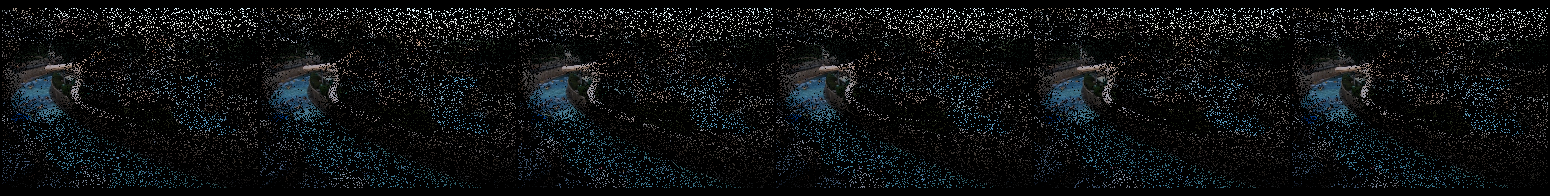
\includegraphics[width=\textwidth]{figures/input.png}\\\vspace{-0.1cm}
    \includegraphics[width=\textwidth]{figures/prediction.png}\\\vspace{-0.1cm}
    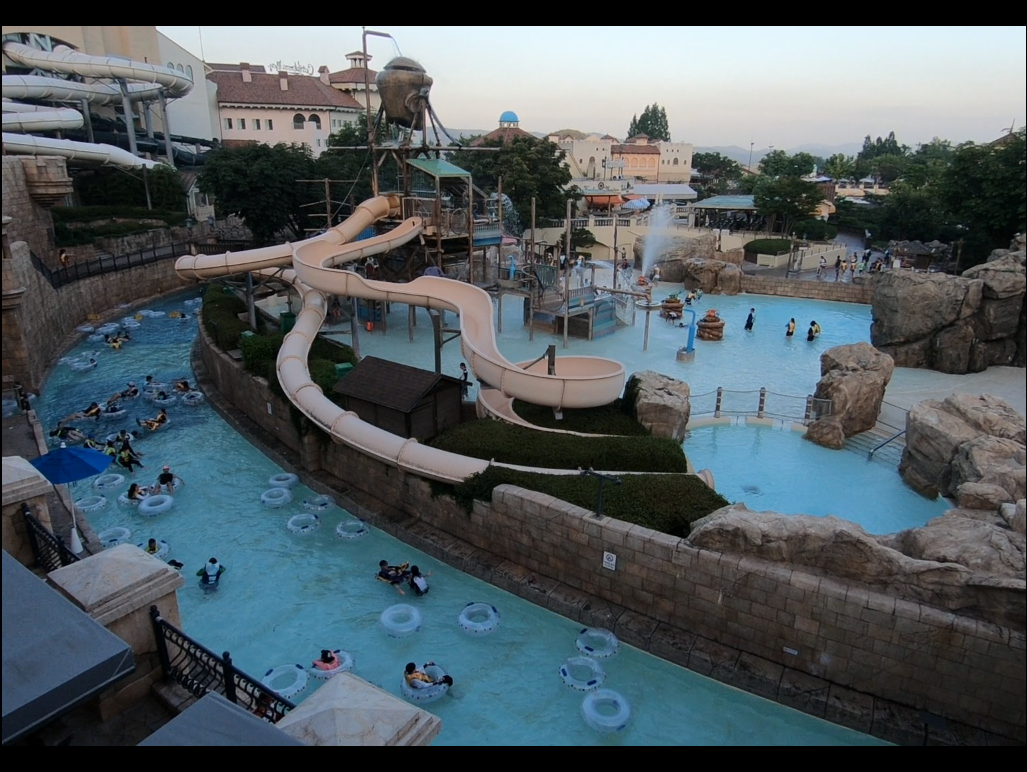
\includegraphics[width=\textwidth]{figures/label.png}\\
    \captionof{figure}{Results of our proposed DeepFovea++ (first setting) framework. The fovea sampled input sequences of low resolution ($192\times 256$) image frames can be seen on the top. The reconstructed super-resolution ($768 \times 1024$) prediction sequence is shown in the middle, and the corresponding label at the bottom.}
    \label{fig:firstresults}
\end{center}%
}]

\begin{abstract} \label{abstract}
Image super-resolution is a well-known problem in the computer vision community. Recent papers extended the problem of super-resolution to videos and showed amazing results. On the other hand deep learning based fovea sampled image reconstruction has drawn some popularity since the DeepFovea publication of Facebook AI. Even though DeepFovea showed outstanding results, the proposed reconstruction network was only able to reconstruct relatively low-resolution images of $128\times128$ pixels. We revisit the proposed DeepFovea architecture to perform fovea sampled video reconstruction and super-resolution ($192 \times 256$ $\to$ $768 \times 1024$) at once. Our proposed architecture, DeepFovea++, first reconstructs a given video sequence by a recurrent U-Net architecture, and afterwards, the desired super-resolution is learned by deformable convolutions. We tested our DeepFovea++ architecture on the challenging REDS dataset. The code is available at {\url{https://github.com/ChristophReich1996/DeepFoveaPP_for_Video_Reconstruction_and_Super_Resolution}}.

\end{abstract}

\section{Introduction} \label{sec:introduction}
A full immersion with virtual reality requires a very high image resolution, a low latency, and a high frame refresh rate \cite{deepfovea}. Kaplanyan \etal \cite{deepfovea} from Facebook Reality Labs approached this problem by making use of the fact that human perception has different levels of visual acuity across the retina. The closer regions in the field of view are to the point of maximum focus - the fovea centralis - the more details from the incoming visual image are perceived. This makes many of the high-level details in image regions that are further away from the fovea point unnecessary, as they are not recognized by the human eye. Instead, the human brain infers this missing visual information based on experience it has made in the past.\\
The authors of DeepFovea \cite{deepfovea} adopted this concept by dropping some of the peripheral pixels for the sake of reduced computational effort. They proposed a deep video reconstruction model that takes such foveated video frames and generates a plausible hypothesis for the missing peripheral pixels based on the remaining ones.\\
In this foveated rendering setup, recorded frames can be masked so that some of the pixels are dropped w.r.t. a probability that is higher the further away the respective pixel is from center of focus. This new masked frame requires less space. They were able to achieve a compression rate of up to 14x without a significant loss in perceived video quality.\\
However, as far as we know, the authors of the DeepFovea paper were working on relatively small images with a resolution of $128\times 128$ pixels. This motivated us to go a step further and add a video super resolution extension to their basic DeepFovea architecture. We trained it in an end-to-end fashion and were able to generate upscaled and reconstructed output frames of a four times higher resolution.\\

\begin{figure*}[htbp!]
    \centering
    \begin{tikzpicture}[xscale=0.6, yscale=0.6, every node/.style={scale=0.625}, >={Stealth[inset=0pt,length=2.8pt,angle'=45]}]
	% Residual enocder block
	\begin{scope}[shift={(0.0,0)}]
		\draw[white, fill=tud0a] (0,-0.5) rectangle++(4.5,5.5);
		\node at (2.25,4.5) {Residual encoder block};
		\draw[tud1c, thick,  ->] (0,2) -- (0.5,2);
		\draw[black, fill=tud2b] (0.5,0.5) rectangle++(0.5,3);
		\node[rotate=90] at (0.75,2) {$3\times 3$ Convolution};
		\draw[tud1c, thick,  ->] (1,2) -- (2,2);
		\draw[black, fill=white] (1.46,2) circle [radius=0.15] node {\begin{tikzpicture}\draw[tud9b] (-0.1, -0.12) -- (0.0, -0.1) -- (0.1, 0.0);\end{tikzpicture}};
		\draw[black, fill=tud2b] (2,0.5) rectangle++(0.5,3);
		\node[rotate=90] at (2.25,2) {$3\times 3$ Convolution};
		\draw[tud1c, thick,  ->] (2.5,2) -- (3.5,2);
		\draw[black, fill=white] (2.73,2) circle [radius=0.15] node {\begin{tikzpicture}\draw[tud9b] (-0.1, -0.12) -- (0.0, -0.1) -- (0.1, 0.0);\end{tikzpicture}};
		\draw[black, fill=white] (3.1,2) circle [radius=0.15] node {$+$};
		\draw[tud1c, thick,  ->] (0.25,2) -- (0.25,0) -- (3.1,0) -- (3.1,1.85);
		\draw[black, fill=tud2b] (3.5,0.5) -- (3.5,3.5) -- (4,3) -- (4,1) -- (3.5,0.5);
		\node[rotate=90] at (3.75,2) {Average pool};
		\draw[tud1c, thick,  ->] (4,2) -- (4.5,2);
	\end{scope}
    
    % Network
    \begin{scope}[shift={(4.6, 2.0)}, xscale=0.625, yscale=0.625]
        \draw[tud1c, thick, ->] (0.0, 0.0) -- (0.5, 0.0);
    	\draw[black, fill=tud0a] (0.5, -3.0) rectangle++ (1.0, 6.0);
    	\node[rotate=90] at (1.0, 0.0) {Res block 1};
    	
    	\draw[tud1c, thick, ->] (1.5, 0.0) -- (2.5, 0.0);
    	\draw[black, fill=tud0a] (2.5, -2.5) rectangle++ (1.0, 5.0);
    	\node[rotate=90] at (3.0, 0.0) {Res block 2};
    	
    	\draw[tud1c, thick, ->] (3.5, 0.0) -- (4.5, 0.0);
    	\draw[black, fill=tud0a] (4.5, -2.0) rectangle++ (1.0, 4.0);
    	\node[rotate=90] at (5.0, 0.0) {Res block 3};
    	
    	\draw[tud1c, thick, ->] (5.5, 0.0) -- (6.5, 0.0);
    	\draw[black, fill=tud0a] (6.5, -1.5) rectangle++ (1.0, 3.0);
    	\node[rotate=90] at (7.0, 0.0) {\small{Res block 4}};	
    	
    	\draw[tud1c, thick, ->] (7.5, 0.0) -- (8.5, 0.0);
    	\draw[black, fill=tud0a] (8.5, -1.0) rectangle++ (1.0, 2.0);
    	\node[rotate=90] at (9.0, 0.0) {\tiny{Res block 5}};
    	
    	\draw[tud1c, thick, ->] (9.5, 0.0) -- (10.5, 0.0);
    	\draw[black, fill=white] (10.0, 0.0) circle [radius=0.2] node {\tiny{c.}};
    	\draw[tud8c, thick, ->] (10.0, 4.5) -- (10.0, 0.25);
    	\draw[black, fill=tud7c!20] (10.5, -1.5) rectangle++ (1.0, 3.0);
    	\node[rotate=90] at (11.0, 0.0) {\tiny{Temp block 1}};
    	\draw[tud8c, thick, ->] (10.5, -1.5) |- (10.0, -2.0) -- (10.0, -4.5);
    	
    	\draw[tud1c, thick, ->] (11.5, 0.0) -- (12.5, 0.0);
    	\draw[black, fill=white] (12.0, 0.0) circle [radius=0.2] node {\tiny{c.}};
    	\draw[tud8c, thick, ->] (12.0, 4.5) -- (12.0, 0.2);
    	\draw[black, fill=tud7c!20] (12.5, -2.0) rectangle++ (1.0, 4.0);
    	\node[rotate=90] at (13.0, 0.0) {\small{Temp block 2}};
    	\draw[tud8c, thick, ->] (12.5, -2.0) |- (12.0, -2.5) -- (12.0, -4.5);
    	
    	\draw[tud1c, thick, ->] (13.5, 0.0) -- (14.5, 0.0);
    	\draw[black, fill=white] (14.0, 0.0) circle [radius=0.2] node {\tiny{c.}};
    	\draw[tud8c, thick, ->] (14.0, 4.5) -- (14.0, 0.25);
    	\draw[black, fill=tud7c!20] (14.5, -2.5) rectangle++ (1.0, 5.0);
    	\node[rotate=90] at (15.0, 0.0) {Temp block 3};
    	\draw[tud8c, thick, ->] (14.5, -2.5) |- (14.0, -3.0) -- (14.0, -4.5);
    	
    	\draw[tud1c, thick, ->] (15.5, 0.0) -- (16.5, 0.0);
    	\draw[black, fill=white] (16.0, 0.0) circle [radius=0.2] node {\tiny{c.}};
    	\draw[tud8c, thick, ->] (16.0, 4.5) -- (16.0, 0.25);
    	\draw[black, fill=tud7c!20] (16.5, -3.0) rectangle++ (1.0, 6.0);
    	\node[rotate=90] at (17.0, 0.0) {Temp block 4};
    	\draw[tud8c, thick, ->] (16.5, -3.0) |- (16.0, -3.5) -- (16.0, -4.5);
    	
    	\draw[tud1c, thick, ->] (17.5, 0.0) -- (18.5, 0.0);
    	\draw[black, fill=tud10a!20] (18.5, -3.5) rectangle++ (1.0, 7.0);
    	\node[rotate=90] at (19.0, 0.0) {Super-resolution block 1};
	
    	\draw[tud1c, thick, ->] (19.5, 0.0) -- (20.5, 0.0);
    	\draw[black, fill=tud10a!20] (20.5, -4.0) rectangle++ (1.0, 8.0);
    	\node[rotate=90] at (21.0, 0.0) {Super-resolution block 2};
    	   
    	\draw[densely dashdotted, tud8c, thick, ->] (22.0, 4.5) -- (22.0, -4.5);
    	\node[black, rotate=90] at (22.35, 0.0) {Time};
    	
    	\draw[densely dashdotted, tud0c, thick, ->] (7.5,-1.5) .. controls (8.5,-2) and (9.5,-2) .. (10.5,-1.5);
    	\draw[densely dashdotted, tud0c, thick, ->] (5.5,-2) .. controls (7.5,-2.5) and (10.5,-2.5) .. (12.5,-2);
    	\draw[densely dashdotted, tud0c, thick, ->] (3.5,-2.5) .. controls (5.5,-3) and (12.5,-3) .. (14.5,-2.5);
    	\draw[densely dashdotted, tud0c, thick, ->] (1.5,-3) .. controls (3.5,-3.5) and (14.5,-3.5) .. (16.5,-3);
    \end{scope}
    
	% Temporal block
	\begin{scope}[shift={(19.0,0)}]
		\draw[white, fill=tud7c!20] (0.0, -0.5) rectangle++ (4.5, 5.5);
		\node at (2.25, 4.5) {Temporal decoder block};
		\draw[tud1c, thick,  ->] (0.0, 2.0) -- (0.5, 2.0);
		\draw[black, fill=tud2b] (0.5, 0.5) rectangle++ (0.5, 3.0);
		\node[rotate=90] at (0.75, 2.0) {$3\times 3$ Convolution};
		\draw[tud1c, thick,  ->] (1.0, 2.0) -- (2.0, 2.0);
		\draw[black, fill=tud2b] (1.1, 1.5) rectangle++ (0.25, 1.0);
		\node[rotate=90] at (1.225, 2.0) {\tiny{Norm.}};
    	\draw[tud8c, thick, ->] (1.6, 2.0) -- (1.6, -0.5);
		\draw[black, fill=white] (1.6,2.0) circle [radius=0.15] node {\begin{tikzpicture}\draw[tud9b] (-0.1, -0.12) -- (0.0, -0.1) -- (0.1, 0.0);\end{tikzpicture}};
		\draw[black, fill=tud2b] (2.0, 0.5) rectangle++ (0.5, 3.0);
		\node[rotate=90] at (2.25, 2.0) {$3\times 3$ Convolution};
		\draw[tud1c, thick,  ->] (2.5, 2.0) -- (3.5, 2.0);
		\draw[black, fill=white] (2.73,2) circle [radius=0.15] node {\begin{tikzpicture}\draw[tud9b] (-0.1, -0.12) -- (0.0, -0.1) -- (0.1, 0.0);\end{tikzpicture}};
		\draw[black, fill=white] (3.1,2) circle [radius=0.15] node {$+$};
		\draw[tud1c, thick,  ->] (0.25, 2.0) -- (0.25, 0.0) -- (3.1,0) -- (3.1, 1.85);
		\draw[black, fill=tud2b] (3.5, 0.5) -- (3.5, 3.5) -- (4.0, 4.0) -- (4.0, 0.0) -- (3.5, 0.5);
		\node[rotate=90] at (3.75, 2.0) {Bilinear upsample};
		\draw[tud1c, thick,  ->] (4.0, 2.0) -- (4.5, 2.0);
	\end{scope}
	
	\begin{scope}[shift={(23.7, 0)}]
	    \draw[white, fill=tud10a!20] (0.0, -0.5) rectangle++ (5.25, 5.5);
    	\node at (2.625, 4.5) {Super-resolution block};
    	\draw[tud1c, thick,  ->] (0.0, 2.0) -- (0.5, 2.0);
    	\draw[black, fill=tud2b] (0.5, 0.5) rectangle++ (0.5, 3.0);
    	\node[rotate=90] at (0.75, 2.0) {$3\times 3$ D. Conv.};
    	\draw[tud1c, thick,  ->] (1.0, 2.0) -- (1.75,2);
    	\draw[black, fill=white] (1.3,2.0) circle [radius=0.15] node {\begin{tikzpicture}\draw[tud9b] (-0.1, -0.12) -- (0.0, -0.1) -- (0.1, 0.0);\end{tikzpicture}};
    	\draw[black, fill=tud2b] (1.75,0.5) -- (1.75,3.5) -- (2.25,4) -- (2.25,0) -- (1.75,0.5);
    	\node[rotate=90] at (2,2) {Bilinear upsample};
    	\draw[tud1c, thick,  ->] (2.25, 2.0) -- (2.75,2);
    	\draw[black, fill=tud2b] (2.75, 0.5) rectangle++ (0.5, 3.0);
    	\node[rotate=90] at (3.0, 2.0) {$3\times 3$ D. Conv.};
    	\draw[tud1c, thick,  ->] (3.25, 2.0) -- (4.25,2);
    	\draw[black, fill=white] (3.5,2.0) circle [radius=0.15] node {\begin{tikzpicture}\draw[tud9b] (-0.1, -0.12) -- (0.0, -0.1) -- (0.1, 0.0);\end{tikzpicture}};
		\draw[black, fill=white] (3.85,2) circle [radius=0.15] node {$+$};
		\draw[tud1c, thick,  ->] (0.25, 2.0) -- (0.25, -0.25) -- (3.85,-0.25) -- (3.85, 1.85);
		\draw[black, fill=tud2b] (4.25, 0.5) rectangle++ (0.5, 3.0);
    	\node[rotate=90] at (4.5, 2.0) {$1\times 1$ D. Conv.};
		\draw[tud1c, thick,  ->] (4.75, 2.0) -- (5.25, 2.0);
	\end{scope}
\end{tikzpicture}

















    \caption{Reconstruction and super-resolution network architecture and the corresponding building blocks of the network in detail.}
    \label{fig:reconstructionnetwork}
\end{figure*}

\section{Previous Work} \label{sec:previouswork}

\subsection{DeepFovea}
The DeepFovea \cite{deepfovea} architecture by Kaplanyan \etal deals with foveated reconstruction i.e. the reconstructions of the most plausible peripheral video from a small portion of the pixels in each frame. This is done by finding the closest matching video. The input videos are foveated in stochastic manner to cover a wide variety. The network design is based on a U-Net i.e. a recurrent video encoder-decoder network with skip connections and is trained in an adversarial manner extending an adversarial loss with spectral normalization, perceptual spatial loss and an optical flow loss. To fit their constraint of being able to reconstruct the video in real-time on a head-mounted display, the network is only trained to reconstruct a $128\times 128$ resolution. The dataset used for training was the YouTube-8M dataset \cite{youtube8m} and contains a variety of natural content including people, animals, nature, \etc

\subsection{Deformable Convolution}
To overcome the geometric limitations of traditional 2d convolutions Dai \etal introduce deformable convolutions \cite{deformableconv1}. Instead of fixed sampling locations, the deformable convolution can learn an offset to the original sampling location. This is done by a separate traditional convolution. This improved operation showed performance benefits in multiple use-cases, like semantic segmentation or object detection. Dai \etal also published an advanced version, deformable convolution v2 \cite{deformableconv}. This operation also learns a modulation mechanism, which further improved the performance of deformable convolutional neural networks. \cite{deformableconv1, deformableconv}\\
The deformable convolution v2 can be expressed by the following formula: 

\begin{equation}
    Y(\Vector{p})=\sum_{k\in K}W_{k}\, X\left(\Vector{p} + \Vector{p}_{k} + \Delta\Vector{p}_{k}\right) \Delta m_{k}.
\end{equation}

Where $\Vector{p}\in\Set{R}^2$ is the current sampling location. Furthermore, $\Vector{p}_{k}^{n\times n}$ represents the indexes of the $n\times n$ convolution kernel. The values $\Delta\Vector{p}_{k}$ and $\Delta m_{k}$ are the learnable offsets, obtained by a separate traditional convolution layer. To be able to sample a position $\Vector{p}\in\Set{R}^2$ from a descried tensor bilinear interpolation us utilized. Finally, the resulting output feature for the position $\Vector{p}$ is represented as $Y\left(\Vector{p}\right)$. \cite{deformableconv}

\subsection{Video Super-resolution}
To achieve good results in video super-resolution, aligning the frames is of great importance. Tao \etal \cite{valillasuperres} introduce a 'sub-pixel motion compensation' layers and incorporate these into an end-to-end convolutional neural network (CNN) framework. Their approach yields an improvement in video super-resolution by '[fusing] multiple frames to reveal image details' 'without the need of parameter tuning'. \cite{valillasuperres}\\

Another approach regarding video super resolution is the attempt by Wang \etal \cite{deformablesuperres} to further improve the aforementioned deformable convolutions towards solving a video restoration task. They propose enhanced deformable convolutions (EDVR) consisting of a pyramid, cascading and deformable alignment modules as well as a temporal and spatial attention fusion module. The former aligns the frames using deformable convolutions in a 'coarse-to-fine manner' and the latter introduces temporal and spatial attention for subsequent restoration. \cite{deformablesuperres}

\subsection{PWC-Net}
PWC-Net \cite{pwcnet} is a CNN model for optical flow estimation, which is widely used in cases where an optical flow prediction is needed. It uses the established principles of pyramidal processing, warping, and the use of a cost volume. PWC-Net utilizes the current optical flow cast into a learnable feature pyramid to warp the CNN features of the second image. These features together with the the features of the first image are then used to construct a cost volume. A CNN is then used to estimate the optical flow on the basis of that volume. This pyramid approach outperformed more traditional encoder-decoder architectures like the famous FlowNet 2 \cite{flownet2} by Nvidia. \cite{pwcnet}

\subsection{General and Adaptive Robust Loss Function} \label{subsec:generaladaptierobustloss}
The adaptive robust loss function by Barron \cite{adaptiveroubustloss} introduces robustness as a continuous parameter. In many deep learning use-cases, loss functions like the L1 or the mean squared error loss are utilized. However, choosing the right supervised loss function can be sometimes very difficult and computationally expensive. Barron introduced an adaptive robust loss function where the shape of the loss is a learnable parameter and thus not require manual tuning anymore. \cite{adaptiveroubustloss}\\

The general loss function Baron introduces, for the input $x=y-\hat{y},\,x\in\Set{R}$, is defined as:
\begin{equation}
    f(x,\alpha,c)=\frac{\abs{\alpha -2}}{\alpha}\left(\left(\frac{\left(x/c\right)^2}{\abs{\alpha-2}}+1\right)^{(\alpha/2)}-1\right).
\end{equation}

Where $\alpha \in \Set{R}$ represents the shape parameter, which controls the robustness of the loss function. Furthermore, the parameter $c\in\Set{R}^+$ controls the size of the loss’s quadratic bowl near $x=0$. \cite{adaptiveroubustloss}\\
This general loss function can be parameterized to match existing loss functions like the mean squared error or the Huber loss. However, to be able to learn the parameters $\alpha$ and $c$ the negative log-likelihood of the probability distribution that corresponds to the generalized loss function. This is needed because if the generalized loss function is optimized directly the loss function will end-up in a trivial solution. \cite{adaptiveroubustloss}\\
Learning the loss function shape showed improved performance in regression tasks like monocular depth estimation. \cite{adaptiveroubustloss}

\section{DeepFovea++ Architecture} \label{sec:architecture}
The DeepFovea++ reconstruction model is mainly based on two parts. First, a recurrent residual U-Net \cite{unet, deepfovea, resunet}, and second, two super-resolution blocks based on deformable convolutions. We train both, the U-Net, and the super-resolution blocks, in an end-to-end setting. The whole reconstruction architecture consists of about 2.3M parameters. We used a relatively small reconstruction model to be able to fit the whole DeepFovea++ framework, consisting of the reconstruction model, a 3d discriminator, and a 3d FFT-discriminator, into GPU memory.

\subsection{Reconstruction and Super-resolution Model} \label{subsec:reconstructionsuperresmodel}
To reconstruct the fovea sampled input image sequence and achieve super-resolution we introduce a recurrent residual U-Net like architecture followed by two super-resolution blocks. Our architecture is highly inspired by the reconstruction network of the original DeepFovea paper. \cite{deepfovea}\\
The recurrent residual U-Net uses five residual blocks in the encoding stage. Each residual block includes two $3\times 3$ convolutions followed by an exponential linear unit (ELU) \cite{elu} activation function, respectively. The final operation of the residual block is an average pooling layer, which downscales the features. The residual mapping is realized by a $1 \times 1$ convolution, to deal with the changing number of feature dimensions.\\
In the encoding path of the recurrent residual U-Net, we utilize four temporal blocks. These include also two $3\times 3$ convolution followed each by an ELU activation function. We introduce a layer normalization \cite{layernorm} operation after the first convolution and store the activated and normalized tensor as the recurrent state. This recurrent tensor is then concatenated in the next forward pass with the input of the corresponding temporal block. This recurrent state can either be reset after each video sequence or be preserved. The recurrent state gets initialized with a random tensors sampled from $\Gaussian{0.0; 0.02}$. To upsample the output of the second convolution of the temporal block, we used a bi-linear upsampling operation. The residual mapping is also implemented in the form of a $1\times 1$ convolution.\\
To achieve the desired super-resolution ($4\times$) we utilize two super-resolution blocks. One super-resolution block consists of two $3\times 3$ deformable convolutions, one bi-linear upsampling layer, two ELU activation functions, and a $1\times 1$ deformable convolution. The residual mapping is utilized with standard $1\times 1$ convolution followed by a bi-linear upsampling layer. We use deformable convolutions to be able to add more spatial details.\\
The whole network, as can be seen in figure \ref{fig:reconstructionnetwork}, consists of 2.3M parameters. This is achieved by 32, 64, 128, 128, and 128 filters in each convolution in the corresponding encoding block. In the encoding blocks, we use 128, 128, 64, and 16 filters in the convolutions. The convolutions in the final super-resolution blocks consist of 8, and 18 filters respectively.

\subsection{Discriminator Models} \label{subsec:discriminator}
We utilize two discriminator networks. The first discriminator network receives the whole 3d video sequence. The second discriminator receives the 3d FFT spectrum of the video sequence, since natural images have characteristic statistics of a vanishing Fourier spectrum. \cite{deepfovea}\\

\begin{figure}[htbp!]
    \centering
    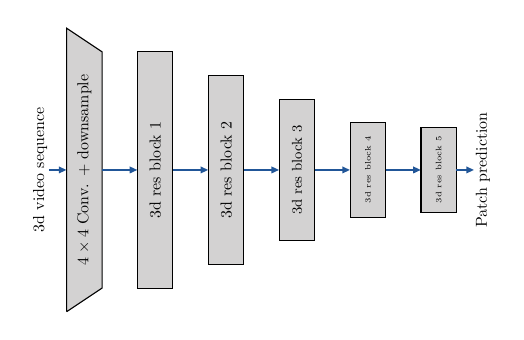
\begin{tikzpicture}[xscale=0.6, yscale=0.75, every node/.style={scale=0.575}, >={Stealth[inset=0pt,length=2.8pt,angle'=45]}]
    \begin{scope}[xscale=0.75, yscale=0.8]
    	\node[rotate=90] at (-0.25, 0.0) {3d video sequence};
    	\draw[tud1c, thick, ->] (0.0, 0.0) -- (0.5, 0.0);
        \draw[black, fill=tud0a] (0.5, -3.0) -- (0.5, 3.0) -- (1.5, 2.5) -- (1.5, -2.5) -- (0.5, -3.0);
        \node[rotate=90] at (1.0, 0.0) {$4 \times 4$ Conv. + downsample};
    	
    	\draw[tud1c, thick, ->] (1.5, 0.0) -- (2.5, 0.0);
    	\draw[black, fill=tud0a] (2.5, -2.5) rectangle++ (1.0, 5.0);
    	\node[rotate=90] at (3.0, 0.0) {3d res block 1};
    	
    	\draw[tud1c, thick, ->] (3.5, 0.0) -- (4.5, 0.0);
    	\draw[black, fill=tud0a] (4.5, -2.0) rectangle++ (1.0, 4.0);
    	\node[rotate=90] at (5.0, 0.0) {3d res block 2};
    	
    	\draw[tud1c, thick, ->] (5.5, 0.0) -- (6.5, 0.0);
    	\draw[black, fill=tud0a] (6.5, -1.5) rectangle++ (1.0, 3.0);
    	\node[rotate=90] at (7.0, 0.0) {\small{3d res block 3}};
    	
    	\draw[tud1c, thick, ->] (7.5, 0.0) -- (8.5, 0.0);
    	\draw[black, fill=tud0a] (8.5, -1.0) rectangle++ (1.0, 2.0);
    	\node[rotate=90] at (9.0, 0.0) {\tiny{3d res block 4}};
    
    	\draw[tud1c, thick, ->] (9.5, 0.0) -- (10.5, 0.0);
    	\draw[black, fill=tud0a] (10.5, -0.9) rectangle++ (1.0, 1.8);
    	\node[rotate=90] at (11.0, 0.0) {\tiny{3d res block 5}};
    	
    	\draw[tud1c, thick, ->] (11.5, 0.0) -- (12.0, 0.0);
    	\node[rotate=90] at (12.25, 0.0) {Patch prediction};
	\end{scope}
\end{tikzpicture}
    \caption{Architecture of the 3d discriminator network.}
    \label{fig:discriminatornetwork}
\end{figure}

The 3d discriminator network, which can be seen in figure \ref{fig:discriminatornetwork}, has the same residual blocks as the reconstruction super-resolution network but uses a 3d convolutions instead of 2d convolutions. A schematic of the residual block can be seen in figure \ref{fig:fftdiscriminatornetwork} (residual encoder block). In each operation, including the learnable parameters, we utilize spectral normalization \cite{spectralnorm} for a more stable adversarial training. To deal with the high-resolution input sequence, we introduce two downsampling operations before the 3d discriminator. First, we used a bi-linear downsampling layer, and second, we utilized a $4\times 4$ convolution. The input sequence that is downscaled by a factor of four at each operation is concatenated and then fed into the 3d discriminator network. The final discriminator is a patch prediction as in \cite{patchgan}.

\begin{figure}[htbp!]
    \centering
    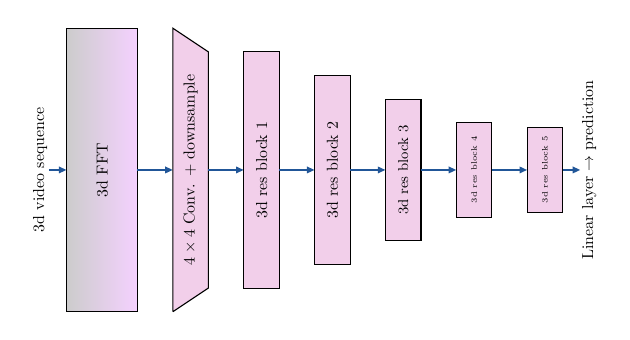
\begin{tikzpicture}[xscale=0.6, yscale=0.75, every node/.style={scale=0.575}, >={Stealth[inset=0pt,length=2.8pt,angle'=45]}]
    \begin{scope}[xscale=0.75, yscale=0.8]
    	\node[rotate=90] at (-3.25, 0.0) {3d video sequence};
    	\draw[tud1c, thick, ->] (-3.0, 0.0) -- (-2.5, 0.0);
    	\shade[black, left color=tud0a, right color=tud10a!20] (-2.5, -3.0) rectangle++ (2.0, 6.0);
    	\draw[black] (-2.5, -3.0) rectangle++ (2.0, 6.0);
        \node[rotate=90] at (-1.5, 0.0) {3d FFT};
    	\draw[tud1c, thick, ->] (-0.5, 0.0) -- (0.5, 0.0);
        \draw[black, fill=tud10a!20] (0.5, -3.0) -- (0.5, 3.0) -- (1.5, 2.5) -- (1.5, -2.5) -- (0.5, -3.0);
        \node[rotate=90] at (1.0, 0.0) {$4 \times 4$ Conv. + downsample};
    	
    	\draw[tud1c, thick, ->] (1.5, 0.0) -- (2.5, 0.0);
    	\draw[black, fill=tud10a!20] (2.5, -2.5) rectangle++ (1.0, 5.0);
    	\node[rotate=90] at (3.0, 0.0) {3d res block 1};
    	
    	\draw[tud1c, thick, ->] (3.5, 0.0) -- (4.5, 0.0);
    	\draw[black, fill=tud10a!20] (4.5, -2.0) rectangle++ (1.0, 4.0);
    	\node[rotate=90] at (5.0, 0.0) {3d res block 2};
    	
    	\draw[tud1c, thick, ->] (5.5, 0.0) -- (6.5, 0.0);
    	\draw[black, fill=tud10a!20] (6.5, -1.5) rectangle++ (1.0, 3.0);
    	\node[rotate=90] at (7.0, 0.0) {\small{3d res block 3}};
    	
    	\draw[tud1c, thick, ->] (7.5, 0.0) -- (8.5, 0.0);
    	\draw[black, fill=tud10a!20] (8.5, -1.0) rectangle++ (1.0, 2.0);
    	\node[rotate=90] at (9.0, 0.0) {\tiny{3d res block 4}};
    
    	\draw[tud1c, thick, ->] (9.5, 0.0) -- (10.5, 0.0);
    	\draw[black, fill=tud10a!20] (10.5, -0.9) rectangle++ (1.0, 1.8);
    	\node[rotate=90] at (11.0, 0.0) {\tiny{3d res block 5}};
    	
    	\draw[tud1c, thick, ->] (11.5, 0.0) -- (12.0, 0.0);
    	\node[rotate=90] at (12.25, 0.0) {Linear layer $\rightarrow$ prediction};
	\end{scope}
\end{tikzpicture}
    \caption{Architecture of the 3d FFT discriminator network.}
    \label{fig:fftdiscriminatornetwork}
\end{figure}

The 3d FFT discriminator network consists of the same architecture as the 3d discriminator model. However, the input video sequence is transformed into a 3d spectrum. Furthermore, the final prediction is produced by a linear layer to achieve a scalar prediction, opposing the patch prediction of the 3d discriminator. \cite{deepfovea}

\subsection{Lossfunction} \label{subsec:lossfunction}
We train our reconstruction and super-resolution network on a weighted sum of multiple loss functions. The full loss function is defined as:

\begin{multline} \label{eq:loss}
    \mathcal{L}=w_{\text{sv}}\,\mathcal{L}_{\text{sv}} + w_{\text{adv}}\,\mathcal{L}_{\text{adv}} + w_{\text{adv fft}}\,\mathcal{L}_{\text{adv fft}}\\
    + w_{\text{flow}}\,\mathcal{L}_{\text{flow}} + w_{\text{LPIPS}}\,\mathcal{L}_{\text{LPIPS}}    
\end{multline}

For the supervised loss $\mathcal{L}_{\text{sv}}$ we used the general and adaptive robust loss function introduced in \ref{subsec:generaladaptierobustloss}.\cite{adaptiveroubustloss} \\
The adversarial loss functions $\mathcal{L}_{\text{adv}}$ and $\mathcal{L}_{\text{adv fft}}$ represents the non-saturating generator GAN loss, which is defined as: \cite{gan}

\begin{equation}
    \mathcal{L}_{\text{adv, adv fft}}=-\Mean{\log \left(\operatorname{D}\left(\hat{\Tensor{I}}\right)\right)}.
\end{equation}

Where $\hat{\Tensor{I}}$ is the reconstructed super-resolution image and $D$ the 3d discriminator or the 3d FFT discriminator. The discriminator networks are trained on the corresponding counter part to the non-saturating generator loss, which is defined as $-\Mean{\log\left(\operatorname{D}\left(\Tensor{I}\right)\right)}-\Mean{\log\left(1-\operatorname{
D}\left(\hat{\Tensor{I}}\right)\right)}$. Where $\Tensor{I}$ is the super-resolution ground truth label. \cite{gan}\\
Besides the supervised and adversarial losses, we also utilized the calibrated perceptual loss (LPIPS) \cite{perceptual} to achieve more natural-looking reconstructed images. 

\begin{equation}
    \mathcal{L}_{\text{LPIPS}} = \frac{1}{5}\sum_{i=1}^{5}\frac{1}{c_{i}\,h_{i}\,w_{i}}\norm{\operatorname{VGG}_{i,2}\left(\hat{\Tensor{I}}\right) - \operatorname{VGG}_{i,2}\left(\Tensor{I}\right)}_{1}
\end{equation}

We take the outputs of the second convolution of the first five blocks of a pre-trained VGG-19 to compute the perceptual loss. This choice is inspired by the original DeepFovea framework. \cite{vgg, deepfovea}

\section{Experiments} \label{sec:experiments}
We trained and tested our DeepFovea++ framework on the famous REalistic and Diverse Scenes (REDS) dataset, which was published in 2019. We analyze the performance of our framework with multiple metrics and discuss the occurring strengths and weaknesses.

\subsection{REDS Dataset} \label{subsec:redsdataset}
In our experiments, we used the REDS dataset \cite{REDS}, which has been compiled in 2019 mainly for the tasks of video deblurring and video super-resolution. It totals $300$ sequences of $100$ high-quality RGB video frames each, with a resolution of $720\times 1280$. These sequences are split into $240$ videos for training, $30$ for validation, and $30$ for testing. However, only the training and test set are publicly available (as of July, 2020). In order to get input-output example pairs for supervised training, we followed the authors of the dataset by downscaling the target high-resolution images by a factor of $4$ to obtain the unmasked low-resolution input frames. However, we used bi-linear instead of bi-cubic interpolation. \cite{REDS}


\subsection{Implementation Details} \label{subsec:implementationdetails}
We implemented the whole DeepFovea++ framework in PyTorch 1.4.0 \cite{pytorch}. Our implementation is based on multiple existing implementations. First, we build our framework on top of the deformable convolution v2 \cite{deformableconv} implementation included in the mmdetection toolbox \cite{mmdetection}. Second, we used the correlation package \cite{flownet2} of Nvidia for implementing the optical flow loss. Furthermore, to estimate the optical flow for the corresponding optical flow loss, we utilized a pre-trained PWC-Net \cite{pwcnet} by Nvidia research. Finally, our main supervised loss function is based on the adaptive robust loss function implementation by Jonathan T. Barron \cite{adaptiveroubustloss}.\\

For optimizing all networks we utilized the Adam optimizer \cite{adam}. For the reconstruction model, we set the learning rate to $3\times 10^{-4}$. The first and second-order running average factors were set 0.1 and 0.95, respectively. In both the 3d discriminator and the 3d FFT-discriminator we set the learning rate to $10^{-4}$. The first and second-order running average factors were set to the same value as for the reconstruction model.\\
To produce the stochastic fovea mask we utilized the following formula.

\begin{equation}
    p_{\Vector{x}} = \begin{cases} 0.98 & \norm{\Vector{x} - \Vector{x}_{\text{f}}}_{2} < 20\\
     0.15 & \norm{\Vector{x} - \Vector{x}_{\text{f}}}_{2} < 40\\
     -0.0415 \norm{\Vector{x} - \Vector{x}_{\text{f}}}_{2} + 1.81 & \norm{\Vector{x} - \Vector{x}_{\text{f}}}_{2} \in \left[20, 40\right]
    \end{cases}
\end{equation}

$p_{\Vector{x}}$ represents the probability that the pixel of the image $\Matrix{I}\in\Set{R}^{3\times\text{height}\times\text{width}}$ at the given position $\Vector{x}=[x_{0}, x_{1}]\in\Set{R}^2$ is not masked out. We mask out the image over all three RGB channels. The vector $\Vector{x}_{f}=[x_{0,f}, x_{1,f}]\in\Set{R}^2$ represent the focus point of the fovea mask. This focus point is randomly generated by 2d uniform distribution which is defined as $\mathcal{U}\left(\left[50, \text{height} - 50\right]; \left[50, \text{width} - 50\right]\right)$. To generate the final fovea mask we sample for each pixel from a uniform distribution $\mathcal{U}\left(0; 1\right)$ and threshold the resulting value with the corresponding $p_{\Vector{x}}$ value to generate a binary mask. This binary mask is then applied to the input image.\\
The preprocessing in our asynchronous data loader contains five steps. In the first step, a batch of high-resolution images ($720 \times 1280$) is loaded to construct a sequence of six frames. Then the images are downscaled by bi-linear interpolation to reach the resolution of $180 \times 320$ pixels. Next, both the inputs and the high-resolution labels are normalized to achieve pixel values between zero and one. Afterward, the fovea mask is generated and applied to the input image. In the final step, the fovea sampled images and the high-resolution label images are cropped and padded to a resolution of $192 \times 256$ and $768 \times 1024$, respectively. This is necessary to match the required input shape of the reconstruction network.\\
We set the weight factors of the loss function \ref{eq:loss} to balance out the magnitudes between the different loss functions. The following weights were used: $w_{\text{sv}}=5$, $w_{\text{adv}}=0.01$, $w_{\text{adv ff}}=0.01$, $w_{\text{flow}}=2$ and $w_{\text{LPIPS}}=1$.
We were able to fit one sequence consisting of six RGB frames on one Tesla V100 (16GB), at training time. We trained our whole framework for 15 epochs on two GPUs with a batch size of two. The training process took us about two days.

\subsection{Results} \label{subsec:results}
For analyzing our framework, results we calculated multiple metrics. First, we compute the common $\operatorname{L1}$ metric and the Mean-Squared-Error (MSE, $\operatorname{L2}$). In case of a reconstructed image $\hat{\Tensor{I}}\in\Set{R}^{c, h, w}$ and the corresponding label $\Tensor{I}\in\Set{R}^{c, h, w}$, the $\operatorname{L1}$ and $\operatorname{L2}$ loss is defined as

\begin{align}
    \operatorname{L1} &= \frac{1}{c\, h\, w}\norm{\hat{\Tensor{I}} - \Tensor{I}}_{1}\\
    \operatorname{L2} &= \frac{1}{c\, h\, w}\norm{\hat{\Tensor{I}} - \Tensor{I}}_{2}.
\end{align}

Additionally we compute the Peak-Signal-To-Noise ($\operatorname{PSNR}$) and the Structural-Similarity-Image-Metric ($\operatorname{SSIM}$) \cite{ssmi} to evaluate quality of prediction. The metrics are defined as follows:

\begin{align}
    \operatorname{PSNR}&=10 \log_{10}\left(\frac{\max\left\{\hat{\Tensor{I}}\right\}^2}{\operatorname{L2}\left(\hat{\Tensor{I}}, \Tensor{I}\right)} \right)\\
    \operatorname{SSIM}&=\frac{4\Mean{\hat{\Tensor{I}}}\Mean{\Tensor{I}}\Cov{\hat{\Tensor{I}}, \Tensor{I}}}{\left(\Mean{\hat{\Tensor{I}}}^2 + \Mean{\Tensor{I}}^2\right)\left(\Var{\hat{\Tensor{I}}} + \Var{\Tensor{I}}\right)}.
\end{align}

We tested our DeepFovea++ framework with two settings. In the first setting, we reset the recurrent state of the reconstruction model after each video. In the second setting, we preserve the recurrent state over the whole training and validation process. Our tests on the REDS dataset \cite{REDS} led to the following results.\\

\begin{table}[!htbp]
    \centering
    \begin{center}
        \begin{tabular}{c|c|c|c|c}
            Rest re. st. & $\operatorname{L1}\downarrow$ & $\operatorname{L2}\downarrow$ & $\operatorname{PSNR}\uparrow$ & $\operatorname{SSIM}\uparrow$ \\ 
            \hline 
            \cmark & 0.0701 & 0.0117 & 22.6681 & 0.9116 \\
            \xmark & {\bf 0.061} & {\bf 0.009} & {\bf 23.8755} & {\bf 0.9290} \\ 
            \hline 
        \end{tabular} 
    \end{center}
    \caption{Validation results of our DeepFovea++ framework on the REDS dataset.}
    \label{tab:results}
\end{table}

From the results in table \ref{tab:results}, it can be observed that resetting the recurrent state leads to a slight drop in performance compared to the setting where no reset is performed. We claim that the reconstruction model can generalize better if the recurrent state is preserved. However, if the recurrent state is not reset, a prediction can possibly depend on a different previous video. This fact could lead to unwanted side effects in predicting the first sequence of a new video.\\
Multiple validation sequences are visualized in the appendix \ref{sec:appendix}. In the visual results, no significant performance difference between the two settings can be observed. 

\section{Conclusion} \label{sec:conclusion}
We propose an architecture to solve the novel problem of fovea sampled reconstruction and video super-resolution. According to our best knowledge, our framework is the first to tackle this problem. We think our framework can be seen as a baseline benchmark for future work. This claim is supported by the qualitative reconstruction results on the natural videos of the REDS dataset.

{\small
    \bibliographystyle{ieee}
    \bibliography{bib}
}

\section{Appendix} \label{sec:appendix}

\begin{figure}[htbp!]
    \centering
    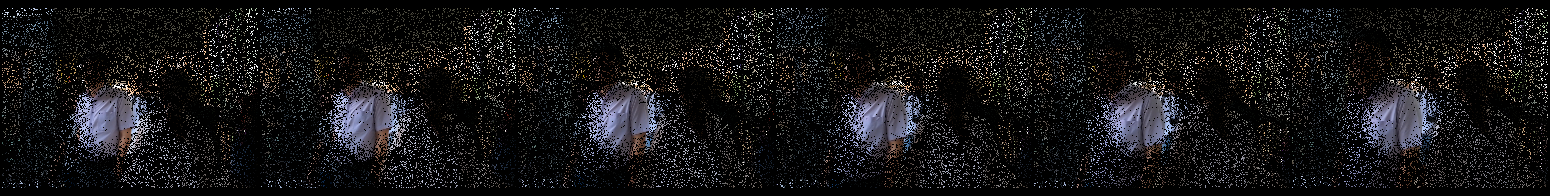
\includegraphics[width=\columnwidth]{figures/rest/input_83_2020-05-04 11_16_57.840082.png}\\\vspace{-0.1cm}
    \includegraphics[width=\columnwidth]{figures/rest/prediction_83_2020-05-04 11_16_53.597074.png}\\\vspace{-0.1cm}
    \includegraphics[width=\columnwidth]{figures/rest/label_83_2020-05-04 11_16_55.895397.png}\\
    \caption{Results of the first DeepFovea++ setting (reset). The fovea sampled input sequences ($192 \times 256$) on the top. The reconstructed super-resolution ($768 \times 1024$) prediction sequence in the middle, and the corresponding label at the bottom.}
    \label{fig:restresults1}
\end{figure}

\begin{figure}[htbp!]
    \centering
    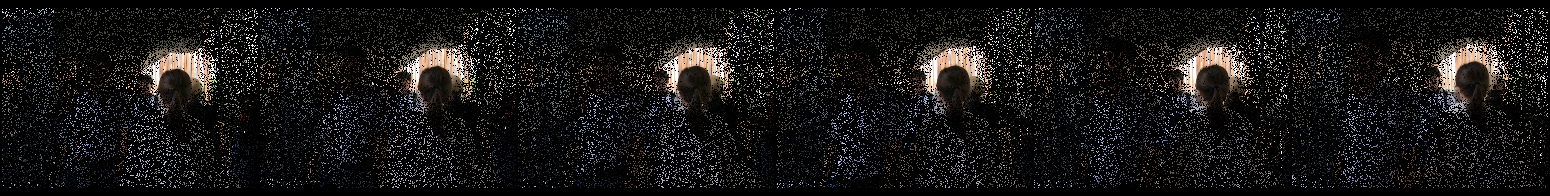
\includegraphics[width=\columnwidth]{figures/no_rest/input_83_2020-05-06 09_56_21.383738.png}\\\vspace{-0.1cm}
    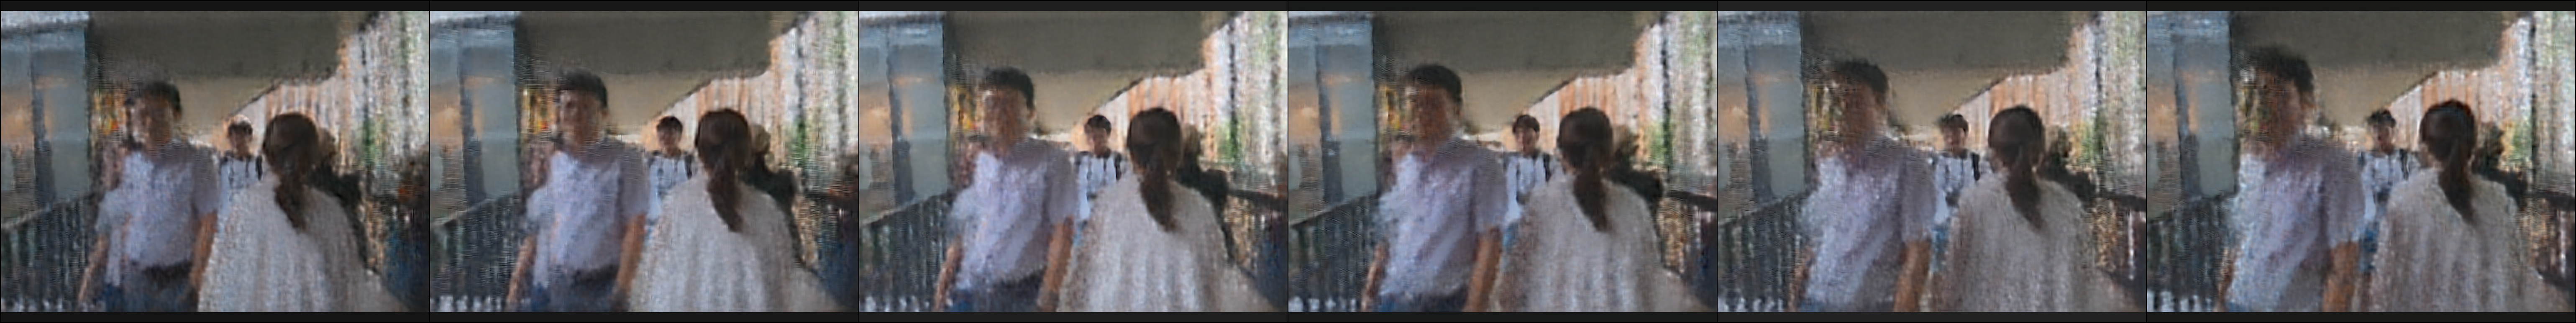
\includegraphics[width=\columnwidth]{figures/no_rest/prediction_83_2020-05-06 09_56_17.234900.png}\\\vspace{-0.1cm}
    \includegraphics[width=\columnwidth]{figures/no_rest/label_83_2020-05-06 09_56_19.447333.png}\\
    \caption{Results of the second DeepFovea++ setting (no reset). The fovea sampled input sequences ($192 \times 256$) on the top. The reconstructed super-resolution ($768 \times 1024$) prediction sequence in the middle, and the corresponding label at the bottom.}
    \label{fig:norestresults1}
\end{figure}

\begin{figure}[htbp!]
    \centering
    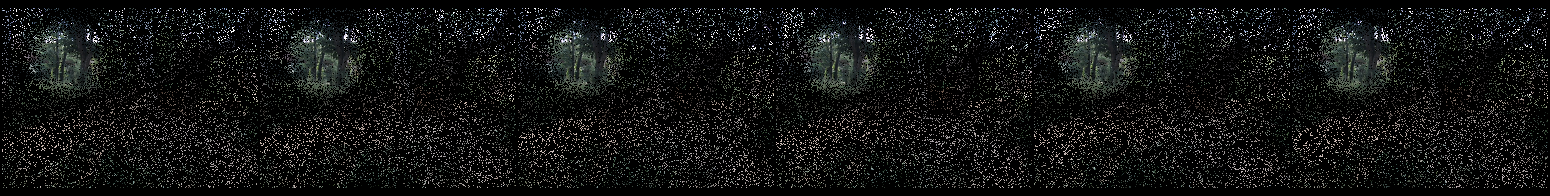
\includegraphics[width=\columnwidth]{figures/rest/input_432_2020-05-04 11_19_22.304534.png}\\\vspace{-0.1cm}
    \includegraphics[width=\columnwidth]{figures/rest/prediction_432_2020-05-04 11_19_18.114088.png}\\\vspace{-0.1cm}
    \includegraphics[width=\columnwidth]{figures/rest/label_432_2020-05-04 11_19_20.713044.png}\\
    \caption{Results of the first DeepFovea++ setting (reset). The fovea sampled input sequences ($192 \times 256$) on the top. The reconstructed super-resolution ($768 \times 1024$) prediction sequence in the middle, and the corresponding label at the bottom.}
    \label{fig:restresults2}
\end{figure}

\begin{figure}[htbp!]
    \centering
    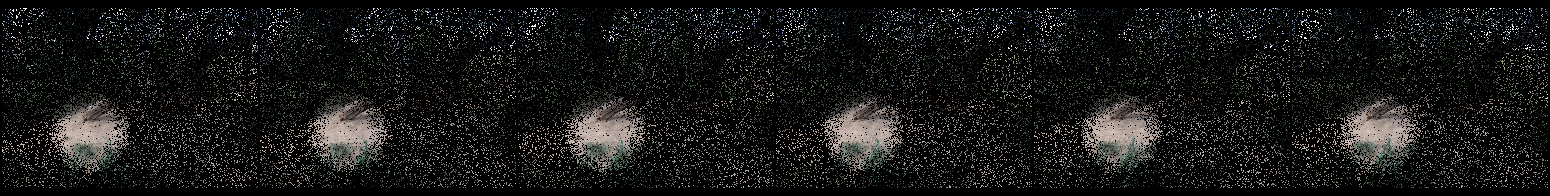
\includegraphics[width=\columnwidth]{figures/no_rest/input_432_2020-05-06 09_58_44.696719.png}\\\vspace{-0.1cm}
    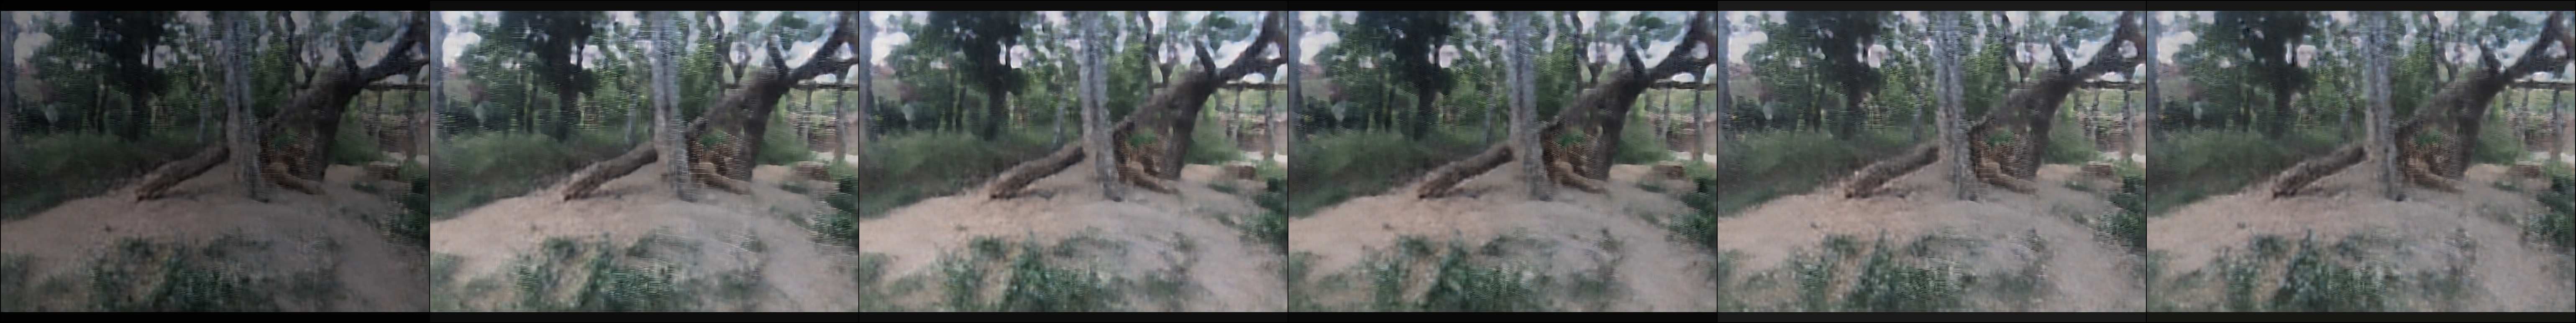
\includegraphics[width=\columnwidth]{figures/no_rest/prediction_432_2020-05-06 09_58_40.811600.png}\\\vspace{-0.1cm}
    \includegraphics[width=\columnwidth]{figures/no_rest/label_432_2020-05-06 09_58_43.122398.png}\\
    \caption{Results of the second DeepFovea++ setting (no reset). The fovea sampled input sequences ($192 \times 256$) on the top. The reconstructed super-resolution ($768 \times 1024$) prediction sequence in the middle, and the corresponding label at the bottom.}
    \label{fig:norestresults2}
\end{figure}

\begin{figure}[htbp!]
    \centering
    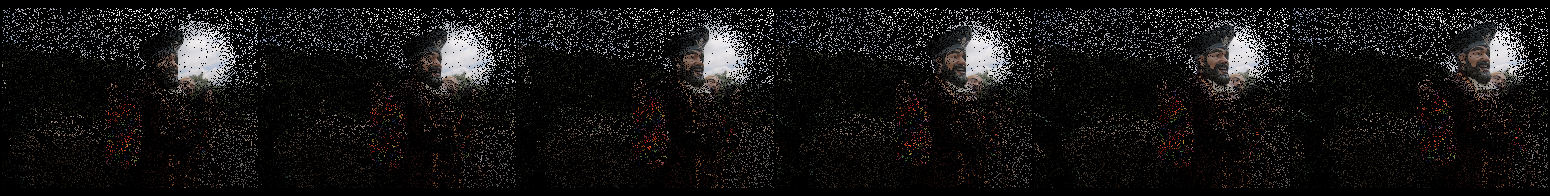
\includegraphics[width=\columnwidth]{figures/rest/input_150_2020-05-04 11_17_29.891315.png}\\\vspace{-0.1cm}
    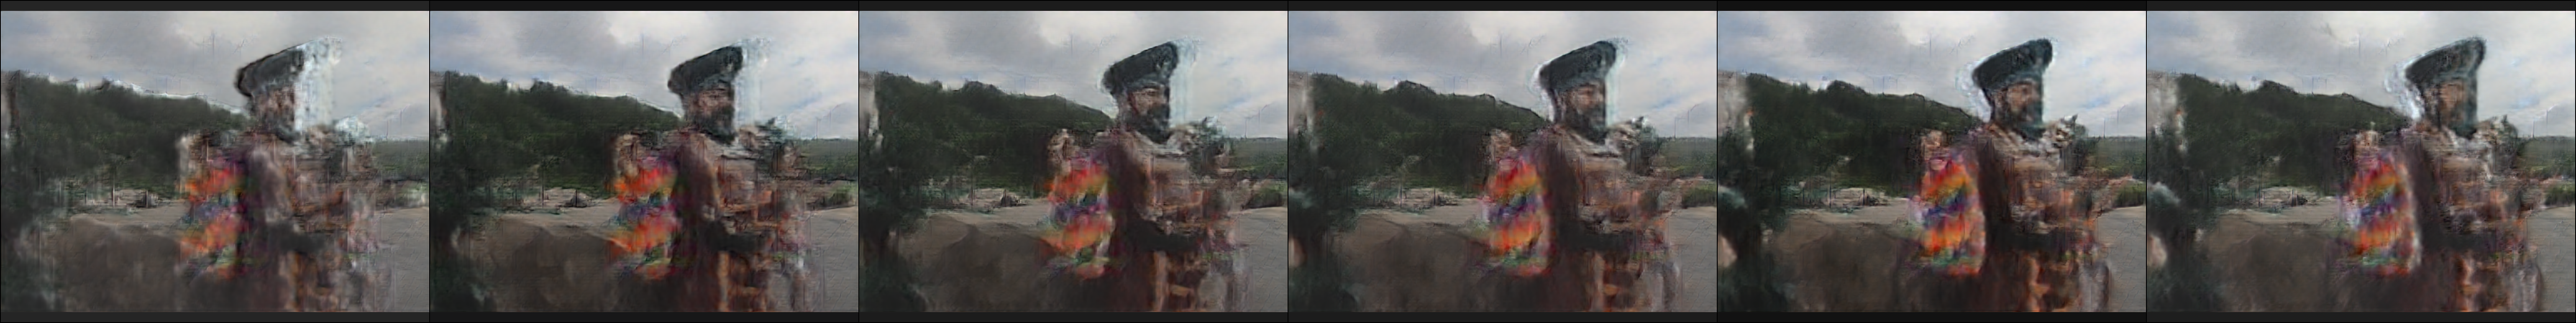
\includegraphics[width=\columnwidth]{figures/rest/prediction_150_2020-05-04 11_17_25.749898.png}\\\vspace{-0.1cm}
    \includegraphics[width=\columnwidth]{figures/rest/label_150_2020-05-04 11_17_27.920524.png}\\
    \caption{Results of the first DeepFovea++ setting (reset). The fovea sampled input sequences ($192 \times 256$) on the top. The reconstructed super-resolution ($768 \times 1024$) prediction sequence in the middle, and the corresponding label at the bottom.}
    \label{fig:restresults3}
\end{figure}

\begin{figure}[htbp!]
    \centering
    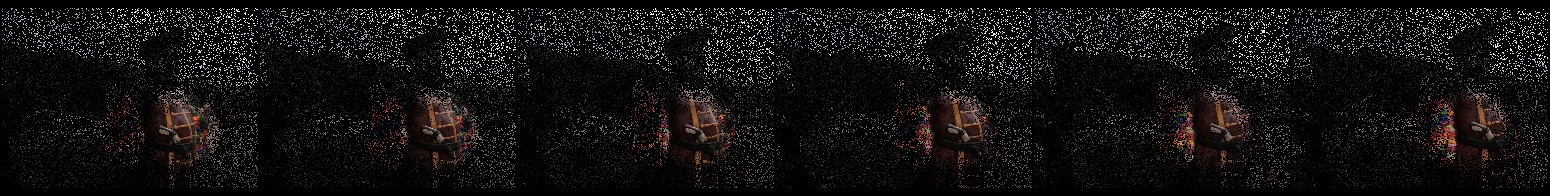
\includegraphics[width=\columnwidth]{figures/no_rest/input_150_2020-05-06 09_56_53.103463.png}\\\vspace{-0.1cm}
    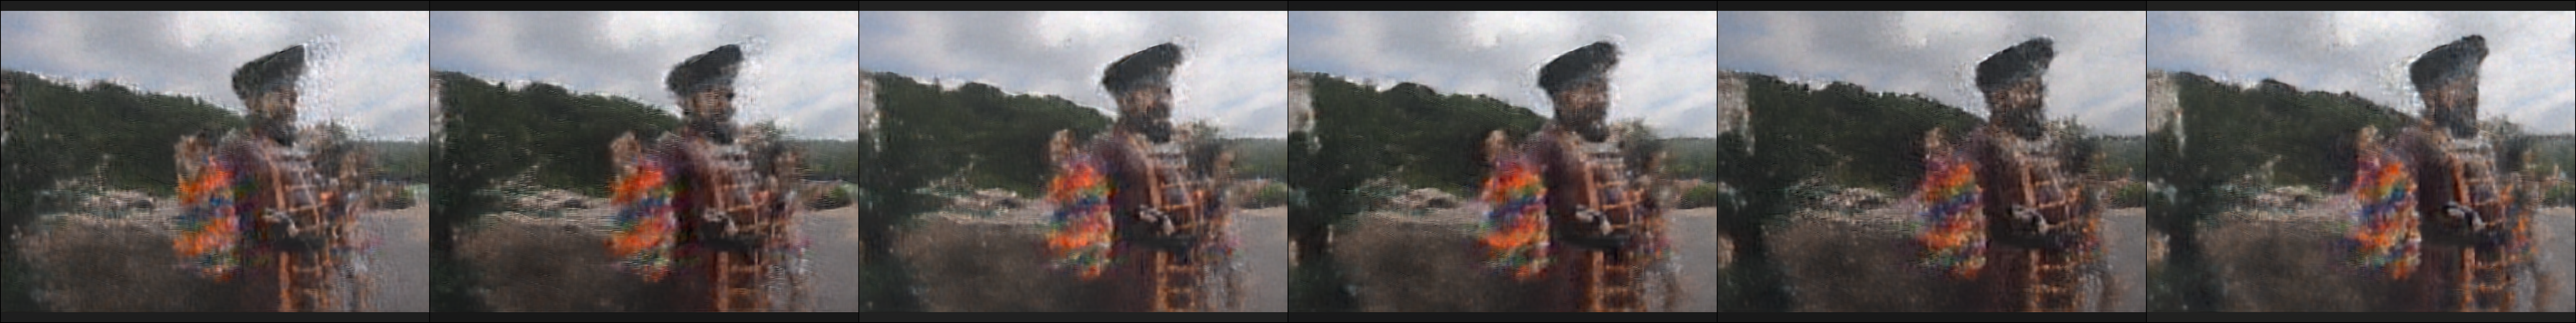
\includegraphics[width=\columnwidth]{figures/no_rest/prediction_150_2020-05-06 09_56_48.941222.png}\\\vspace{-0.1cm}
    \includegraphics[width=\columnwidth]{figures/no_rest/label_150_2020-05-06 09_56_51.153540.png}\\
    \caption{Results of the second DeepFovea++ setting (no reset). The fovea sampled input sequences ($192 \times 256$) on the top. The reconstructed super-resolution ($768 \times 1024$) prediction sequence in the middle, and the corresponding label at the bottom.}
    \label{fig:norestresults3}
\end{figure}

\vfill

\end{document}